% =============================================================================
%  A Comparative Study of Hard-Constrained Price-Domain Networks and
%  Native Volatility-Domain Networks for the IV Surface
% =============================================================================
\documentclass[11pt,a4paper]{article}

\usepackage[utf8]{inputenc}
\usepackage[T1]{fontenc}
\usepackage{lmodern}
\usepackage{amsmath,amssymb,amsthm}
\usepackage{mathtools}
\usepackage{booktabs}
\usepackage{multirow}
\usepackage{graphicx}
\usepackage[margin=1in]{geometry}
\usepackage{hyperref}
\usepackage{cleveref}
\usepackage{natbib}
\usepackage{subcaption}
\usepackage{xcolor}
\usepackage{bm}
\usepackage{float}
\usepackage{enumitem}
\usepackage{tabularx}
\usepackage{array}
\usepackage{tikz}
\usetikzlibrary{positioning,arrows.meta,shapes.geometric,fit,backgrounds,calc}

\graphicspath{{figs/}}

\newcommand{\iv}{\sigma_{\mathrm{IV}}}
\newcommand{\logm}{k}
\DeclareMathOperator{\diag}{diag}

\tikzset{
  block/.style  = {draw, rounded corners, thick, align=center, minimum height=0.9cm,
                   minimum width=2.4cm, fill=blue!5, font=\small},
  data/.style   = {draw, thick, align=center, minimum height=0.8cm,
                   minimum width=2.0cm, fill=yellow!15, font=\small},
  model/.style  = {draw, rounded corners, thick, align=center, minimum height=1.0cm,
                   minimum width=2.6cm, fill=green!8, font=\small},
  loss/.style   = {draw, thick, align=center, minimum height=0.7cm,
                   minimum width=1.8cm, fill=red!8, rounded corners=2pt, font=\small},
  hyper/.style  = {draw, rounded corners, thick, align=center, minimum height=1.0cm,
                   minimum width=2.6cm, fill=purple!8, font=\small},
  arrow/.style  = {-Stealth, thick},
  dashedarrow/.style = {-Stealth, thick, dashed},
}

\title{Hard Price-Domain Constraints vs.\ Native Volatility-Domain Models \\
       for the Implied-Volatility Surface: \\
       \large An Empirical Comparison of ISNN, HyperIV, HyperISNN and SSVI}

\author{Parshv Joshi \\
        \small Under the mentorship of Prof.\ Abhishek Tilva}
\date{April 2026}

% =============================================================================
\begin{document}
\maketitle

\begin{abstract}
We study four families of models for the S\&P~500 implied-volatility (IV)
surface and ask a question that, to our knowledge, has not been answered
under one experimental protocol: \emph{how do hard-constrained
price-domain networks compare against native volatility-domain models, both
in accuracy and in compute?} The four pipelines are: (A) the per-day
Input-Specified Neural Network (ISNN-2) of \citet{jadoon2025isnn} fit on
normalized call prices; (B) HyperIV \citep{yang2025hyperiv}, a
Set-Transformer hyper-network that emits the weights of a tiny IV-MLP;
(C) HyperISNN, a novel residual hyper-network of our own design that
generates the strictly-positive weights of an ISNN-2 from a reference set;
and (D) the SSVI parametric surface of \citet{gatheral2014ssvi}, calibrated
once per day. All four are trained and evaluated on the same Moussa-filtered
\citep{moussa2025arbitrage} OptionMetrics quote set (1\,762 SPX days,
2013--2019). We find that SSVI is the most accurate (test IV RMSE
$0.00774$) but takes a per-day L-BFGS-B fit; HyperIV is a close second
($0.0131$) and is roughly $500\times$ faster at inference than SSVI's
per-day calibration. The two price-domain pipelines (ISNN, HyperISNN)
guarantee static no-arbitrage by construction but are materially less
accurate, both in IV and, surprisingly, in their \emph{native} price
domain --- inverting their predictions through Black--Scholes to IV and
back to price gives smaller dollar errors than reading prices off the
network directly. HyperISNN is less accurate than ISNN but two orders of
magnitude faster, illustrating the general amortisation argument for
hyper-networks in finance.
\end{abstract}

\tableofcontents
\bigskip

% =============================================================================
\section{Motivation and Objective}
\label{sec:motivation}

\subsection{Why this comparison is missing in the literature}

The implied-volatility surface $\iv(K, T)$ is the central object of equity
derivatives modelling: it summarises every European option price into a
two-dimensional smooth function from which traders read skew, term structure
and risk-neutral densities. Three communities have produced largely
non-overlapping literatures around fitting this surface:

\begin{enumerate}[leftmargin=*,itemsep=2pt,topsep=2pt]
  \item \textbf{Parametric arbitrage-free models} (e.g., SVI / SSVI of
        \citet{gatheral2004svi,gatheral2014ssvi}), which fit a small handful
        of parameters per day under tight no-arbitrage constraints.
  \item \textbf{Hard-constrained neural surrogates} that fit a network
        directly on \emph{prices} and rely on architectural constraints
        (positivity of certain weights, monotone activations) to guarantee
        absence of static arbitrage. The Input-Specified Neural Network
        (ISNN-2) of \citet{jadoon2025isnn} is the most recent published
        representative of this family, building on the input-convex
        construction of \citet{amos2017icnn}.
  \item \textbf{Volatility-domain hyper-networks} that train a
        permutation-invariant encoder once on years of data and, at
        inference, generate per-day target-network weights from a small
        reference set of quotes. HyperIV \citep{yang2025hyperiv} is the
        recent prototype; it follows the hyper-network template of
        \citet{ha2017hypernetworks} with a Set Transformer
        \citep{lee2019set} encoder.
\end{enumerate}

These three families make very different trade-offs. (1)~SSVI is highly
interpretable and arbitrage-free, but every new day requires a fresh
non-convex fit. (2)~ISNN-style networks output an arbitrage-free price
surface by construction but, because they are trained per-day on
\emph{normalized prices}, their loss is dominated by deep ITM intrinsic
value and they typically have poor IV-domain behaviour. (3)~HyperIV
amortises the per-day fit into a one-time training cost, which on inference
collapses to a single forward pass; it operates directly in IV-space and
adds soft penalties for static no-arbitrage. To our knowledge, no published
study has put all three families on the same dataset, the same evaluation
points, the same arbitrage filter and the same Phase-1/Phase-2 protocol. The
motivation of this work is to do exactly that, and to design a fourth
pipeline --- \emph{HyperISNN} --- that bridges the price-domain hard-
constrained family with the hyper-network amortisation argument: a
hyper-network that emits the strictly-positive weights of an ISNN-2.

\subsection{Concrete objectives}

\begin{enumerate}[leftmargin=*,itemsep=2pt,topsep=2pt]
  \item Build a single, reproducible pipeline that ingests raw OptionMetrics
        SPX EOD quotes, applies a real-time arbitrage filter
        \citep{moussa2025arbitrage}, and exposes a unified per-day quote
        store consumed by all four pipelines.
  \item Implement Pipelines A--D under one PyTorch / SciPy stack and one
        configuration system, so that hyper-parameters, train/val/test
        splits, and evaluation grids are shared.
  \item Run a Phase-1 (same-day fit) and Phase-2 (next-day VolGAN-driven
        prediction \citep{cont2025volgan}) evaluation, in both IV-space and
        BS-implied dollar price.
  \item Provide a wall-clock comparison: \emph{per-day fit} (ISNN, SSVI)
        vs.\ \emph{amortised inference} (HyperIV, HyperISNN), so that the
        downstream user can pick a model based on accuracy/latency budget.
  \item Diagnose, in detail, why hard-constrained price-domain networks
        fail to dominate even the simple parametric SSVI surface, despite
        their structural arbitrage guarantees.
\end{enumerate}

% =============================================================================
\section{Literature Study}
\label{sec:lit}

We review only the four works on which this comparison is built; the
broader IV-surface modelling literature is summarised, e.g., in
\citet{ackerer2020deep} and \citet{boursin2024operator}.

\paragraph{Moussa (2025) --- Real-time arbitrage filter
\citep{moussa2025arbitrage}.} Moussa proposes a one-pass linear-program
filter that, for each day, removes the minimal set of mid-quotes whose
removal makes the residual surface satisfy static no-arbitrage:
intrinsic-value bounds, calendar monotonicity, and butterfly convexity. The
filter is parameter-free and runs in milliseconds per day, which is what
makes it usable as a preprocessor for downstream learners. We adopt it
as the \emph{only} cleaning step before any model sees the data, so that
all four pipelines train on identical inputs and are graded against the
filter's projected mid-prices.

\paragraph{Gatheral \& Jacquier (2014) --- Arbitrage-free SSVI
\citep{gatheral2014ssvi}.} SSVI is a five-parameter total-variance surface
$w(k, t) = \tfrac{\theta(t)}{2}\bigl(1 + \rho \phi(\theta) k +
\sqrt{(\phi k + \rho)^2 + (1-\rho^2)}\bigr)$ with a power-law
$\phi(\theta) = \eta / \sqrt{\theta}$ and a three-parameter ATM
term-structure $\theta(t) = a + b t^{c}$. Sufficient inequality conditions
on $(\rho, \eta, c)$ guarantee absence of butterfly and calendar arbitrage
across the entire surface. We use the \citet{gatheral2014ssvi}
parameterisation throughout, fitted per-day with L-BFGS-B over $10$ random
restarts (cf.\ \citet{corbetta2018ssvi} for the rationale on multi-restart
SSVI calibration).

\paragraph{Jadoon et al.\ (2025) --- ISNN-2 \citep{jadoon2025isnn}.}
ISNN-2 is an input-convex / input-monotone network for the option price
surface, derived from \citet{amos2017icnn}. Two scalar inputs --- normalized
strike $x_0 = K/F$ and time-to-maturity $t_0 = T$ --- are processed in two
separate branches that exchange information through skip connections;
strictly-positive weights enforced by softplus parameterisation guarantee
that the output is convex in $K$ (no butterfly arbitrage) and monotone in
$T$ (no calendar arbitrage). The network is trained per-day with MSE on
normalized call prices. We re-implement ISNN-2 with the corrections
documented in our code (forward-measure normalisation, $\beta=1$ softplus,
proper post-step weight projection).

\paragraph{Yang et al.\ (2025) --- HyperIV \citep{yang2025hyperiv}.} HyperIV
is a Set-Transformer-based \citep{lee2019set,vaswani2017attention}
hyper-network: a small permutation-invariant encoder $g_\theta$ ingests a
$9$-element \emph{reference set} $Z_t$ of recent contracts and emits the
$337$ weights of a tiny IV-MLP $h_\omega : (k, T) \mapsto \iv$. Training is
amortised across years of data with MSE on IV plus three soft arbitrage
penalties (calendar, butterfly $g$-function, Durrleman integral
\citep{durrleman2010g}). At inference, a single forward pass through
$g_\theta$ yields the per-day weights $\omega_t$; querying the surface at
any $(k, T)$ then costs only an MLP evaluation of $h_{\omega_t}$.

\paragraph{Other related work.} VolGAN \citep{cont2025volgan} provides the
generative next-day surface model used in our Phase-2 evaluation; the
input-convex construction goes back to \citet{amos2017icnn};
hyper-networks generally to \citet{ha2017hypernetworks}; for end-to-end
deep IV smoothing, \citet{ackerer2020deep,boursin2024operator,
chataigner2020dlv} are the closest references.

% =============================================================================
\section{Technical Details: Design and Implementation}
\label{sec:tech}

\subsection{End-to-end pipeline}

\begin{figure}[H]
\centering
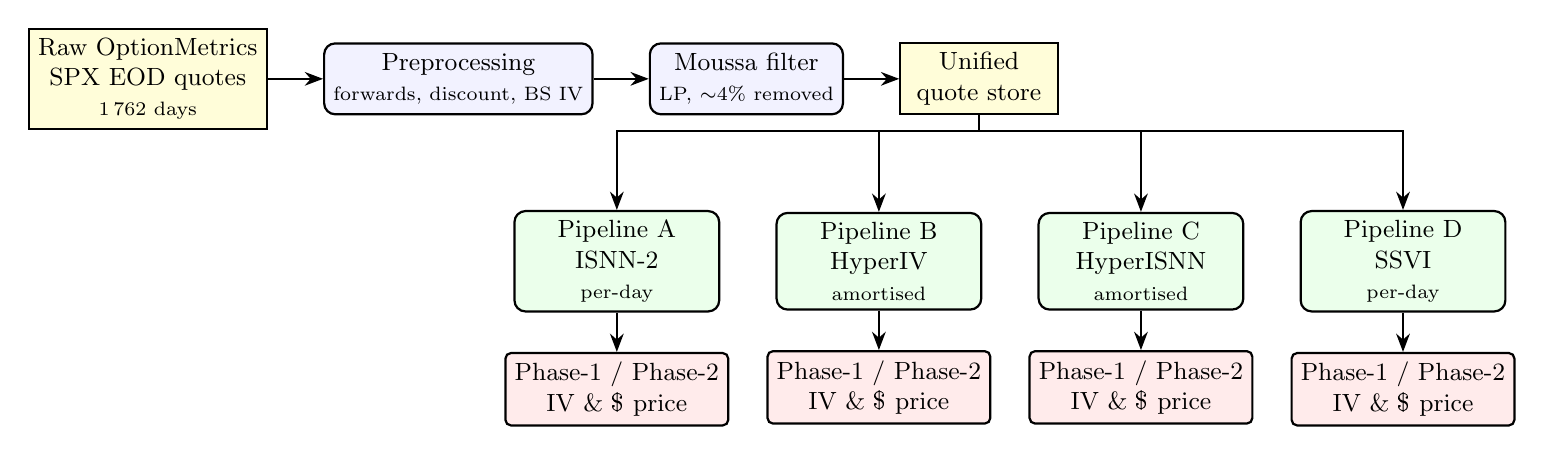
\begin{tikzpicture}[node distance=0.5cm and 0.7cm]
  \node[data]  (raw)   {Raw OptionMetrics \\ SPX EOD quotes \\ \scriptsize 1\,762 days};
  \node[block, right=of raw] (pre) {Preprocessing \\ \scriptsize forwards, discount, BS IV};
  \node[block, right=of pre] (mou) {Moussa filter \\ \scriptsize LP, $\sim$4\% removed};
  \node[data,  right=of mou] (uni) {Unified \\ quote store};
  \draw[arrow] (raw)  -- (pre);
  \draw[arrow] (pre) -- (mou);
  \draw[arrow] (mou) -- (uni);

  \node[model, below=1.2cm of uni, xshift=-4.6cm] (A) {Pipeline A\\ ISNN-2\\ \scriptsize per-day};
  \node[model, right=of A] (B) {Pipeline B\\ HyperIV\\ \scriptsize amortised};
  \node[model, right=of B] (C) {Pipeline C\\ HyperISNN\\ \scriptsize amortised};
  \node[model, right=of C] (D) {Pipeline D\\ SSVI\\ \scriptsize per-day};

  \draw[arrow] (uni.south) -- ++(0,-0.2) -| (A.north);
  \draw[arrow] (uni.south) -- ++(0,-0.2) -| (B.north);
  \draw[arrow] (uni.south) -- ++(0,-0.2) -| (C.north);
  \draw[arrow] (uni.south) -- ++(0,-0.2) -| (D.north);

  \node[loss, below=of A] (eA) {Phase-1 / Phase-2 \\ IV \& \$ price};
  \node[loss, below=of B] (eB) {Phase-1 / Phase-2 \\ IV \& \$ price};
  \node[loss, below=of C] (eC) {Phase-1 / Phase-2 \\ IV \& \$ price};
  \node[loss, below=of D] (eD) {Phase-1 / Phase-2 \\ IV \& \$ price};
  \draw[arrow] (A) -- (eA);
  \draw[arrow] (B) -- (eB);
  \draw[arrow] (C) -- (eC);
  \draw[arrow] (D) -- (eD);
\end{tikzpicture}
\caption{End-to-end pipeline. Raw OptionMetrics quotes are run through a
shared preprocessing stage (forward-curve and discount-curve materialisation,
Black--Scholes IV inversion) and then through the Moussa arbitrage filter,
which produces the unified quote store consumed by all four models.}
\label{fig:pipeline}
\end{figure}

\subsection{Pipeline A --- ISNN-2 (per-day price-domain)}
\label{sec:pipeA}

\paragraph{Architecture.} Following \citet{jadoon2025isnn}, two scalar
inputs --- normalized strike $x_0 = K/F$ and time-to-maturity $t_0$ --- are
fed into a $H{=}64$-wide, $L{=}3$-deep two-branch network:
\begin{align*}
  t_{h+1} &= \sigma_m\!\bigl(t_h W^{tt}_h + b^t_h\bigr), \\
  x_1     &= \sigma_{mc}\!\bigl(x_0 W^{xx_0}_0 + t_0 W^{xt}_0 + b^x_0\bigr), \\
  x_{h+1} &= \sigma_{mc}\!\bigl(x_h W^{xx}_h + x_0 W^{xx_0}_h + t_h W^{xt}_h + b^x_h\bigr),
\end{align*}
where $\sigma_{mc}$ and $\sigma_m$ are softplus, $W^{xx}, W^{xt}, W^{tt}$
are non-negative (enforced by clamping after every optimizer step), and
$W^{xx_0}$ are unconstrained skip connections that preserve convexity. The
output is the normalized call $C/S = W^{\mathrm{out}}_+ \, x_L$. Convexity
of $C$ in $K$ (no butterfly arbitrage) and monotonicity in $T$ (no calendar
arbitrage) are guaranteed by construction.

\paragraph{Loss / training.} MSE on $C/S$, optimizer Adam at LR $10^{-2}$,
$2{,}000$ epochs. A separate ISNN is fit for every trading day (one network
per day, $\sim$$2{,}500$ parameters).

\paragraph{Regularisation.} Hard structural constraint via
\texttt{NonNegativeLinear} forward-pass clamp and softplus output. AdamW
$L_2$ weight decay plays a secondary role.

\subsection{Pipeline B --- HyperIV (amortised IV-domain)}
\label{sec:pipeB}

\begin{figure}[H]
\centering
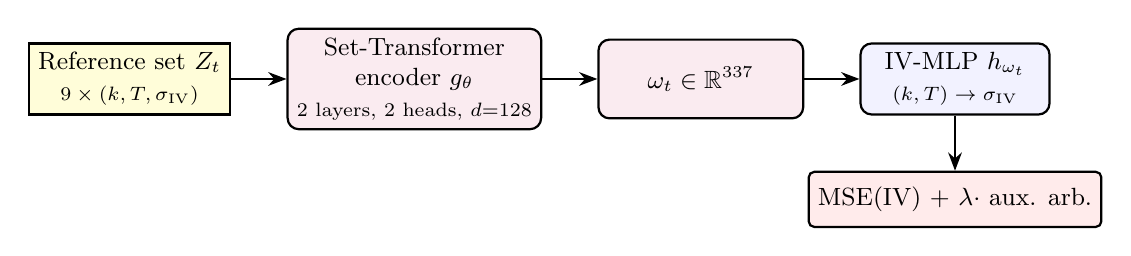
\begin{tikzpicture}[node distance=0.4cm and 0.7cm]
  \node[data] (Z) {Reference set $Z_t$ \\ \scriptsize $9 \times (k, T, \iv)$};
  \node[hyper, right=of Z] (enc) {Set-Transformer \\ encoder $g_\theta$ \\ \scriptsize 2 layers, 2 heads, $d{=}128$};
  \node[hyper, right=of enc] (om)  {$\omega_t \in \mathbb{R}^{337}$};
  \node[block, right=of om] (h)   {IV-MLP $h_{\omega_t}$ \\ \scriptsize $(k, T) \to \iv$};
  \node[loss,  below=0.7cm of h] (l) {MSE(IV) + $\lambda \cdot$ aux. arb.};
  \draw[arrow] (Z) -- (enc); \draw[arrow] (enc) -- (om); \draw[arrow] (om) -- (h);
  \draw[arrow] (h) -- (l);
\end{tikzpicture}
\caption{Pipeline B (HyperIV). The same trained $g_\theta$ is used on every
day; only the reference set $Z_t$ changes.}
\end{figure}

\paragraph{Architecture.} Set-Transformer encoder
\citep{lee2019set,vaswani2017attention} with hidden $d{=}128$, $2$ heads,
$2$ encoder layers; mean-pool $\to$ MLP head $\to$ $\omega_t \in
\mathbb{R}^{337}$, which are reshaped into the weights of a tiny IV-MLP
$h_{\omega_t} : (k, T) \mapsto \iv$.

\paragraph{Loss / training.} MSE on $\iv$ over a subsampled set of
$N_c = 1024$ contracts per day, plus an auxiliary arbitrage loss with three
components: a calendar-spread penalty, a butterfly $g$-function penalty
\citep{roper2010arbitrage}, and a Durrleman integral penalty
\citep{durrleman2010g}. Optimizer Adam at LR $10^{-3}$, batch $128$,
$500$ epochs, cosine-annealing to $10^{-5}$.

\paragraph{Reference set.} We use the corrected anchor selector that
targets positive call deltas $\{0.75, 0.50, 0.25\}$ at three short
maturities and three long maturities, padded to $9$ if fewer eligible
contracts are available. This is the only modification to the original
\citet{yang2025hyperiv} recipe.

\subsection{Pipeline C --- HyperISNN (residual hyper-network for ISNN
weights)}
\label{sec:pipeC}

This pipeline is novel and the implementation that we ship deviates
materially from a naive ``hyper-network outputs ISNN weights'' design.

\begin{figure}[H]
\centering
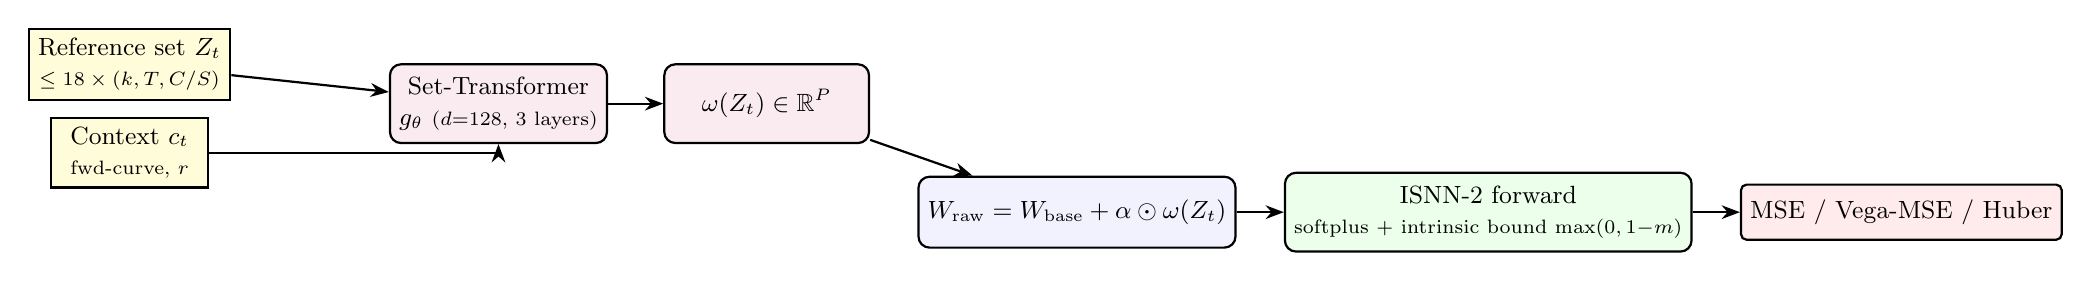
\begin{tikzpicture}[node distance=0.4cm and 0.7cm]
  \node[data] (Z) {Reference set $Z_t$ \\ \scriptsize $\le 18 \times (k, T, C/S)$};
  \node[data, below=0.2cm of Z] (ctx) {Context $c_t$ \\ \scriptsize fwd-curve, $r$};
  \node[hyper, right=2.0cm of Z, yshift=-0.5cm] (enc) {Set-Transformer\\$g_\theta$ \scriptsize ($d{=}128$, 3 layers)};
  \node[hyper, right=of enc] (om)  {$\omega(Z_t) \in \mathbb{R}^P$};
  \node[block, below right=0.4cm and 0.6cm of om] (mix)
       {$W_{\mathrm{raw}} = W_{\mathrm{base}} + \alpha \odot \omega(Z_t)$};
  \node[model, right=0.6cm of mix] (isnn)
       {ISNN-2 forward \\ \scriptsize softplus + intrinsic bound $\max(0, 1{-}m)$};
  \node[loss,  right=0.6cm of isnn] (l) {MSE / Vega-MSE / Huber};
  \draw[arrow] (Z) -- (enc); \draw[arrow] (ctx) -| (enc);
  \draw[arrow] (enc) -- (om); \draw[arrow] (om) -- (mix);
  \draw[arrow] (mix) -- (isnn); \draw[arrow] (isnn) -- (l);
\end{tikzpicture}
\caption{Pipeline C (HyperISNN). $W_{\mathrm{base}}$ and the per-parameter
modulation scale $\alpha$ are shared across all days; only $\omega(Z_t)$ is
day-specific.}
\end{figure}

\paragraph{Residual weight generation.} For each day $t$ we form
\[
W_{\mathrm{raw}}(t) \;=\; W_{\mathrm{base}} \;+\; \alpha \odot \omega(Z_t,c_t),
\qquad
W_{\mathrm{ISNN}} \;=\; \mathrm{softplus}(W_{\mathrm{raw}}) + \varepsilon
\]
on every entry that the ISNN architecture requires to be positive. Here
$W_{\mathrm{base}} \in \mathbb{R}^P$ are learnable mean ISNN weights, shared
across days; $\alpha \in \mathbb{R}^P$ is a per-parameter learnable
modulation scale (initialised to $0.1$); $\omega(Z_t, c_t) \in \mathbb{R}^P$
is produced by a Set-Transformer hyper-network from the day's reference set
$Z_t$ and a forward-curve / rate context vector $c_t$. The shared output
bias $b^{\mathrm{out}}$ is also a single learnable scalar.

\paragraph{Hard intrinsic-value floor.} We add the forward-measure
intrinsic bound $\max(0, 1 - m)$ \emph{inside} the ISNN forward pass, so
that the output is $C/S \ge \max(0, 1 - m)$ by construction. (The original
spec used the spot-measure bound $1 - m e^{-rT}$, which our code corrects.)

\paragraph{Warm-up training.} A two-phase schedule is critical for
stability: in the first $500$ of $10{,}000$ steps, the hyper-network and
$\alpha$ are \emph{frozen} ($\omega$ is multiplied by zero) so that only
$W_{\mathrm{base}}$ and $b^{\mathrm{out}}$ train --- this finds a sensible
``mean'' ISNN surface. The hyper-network and $\alpha$ are then unfrozen
and the entire model trains jointly. The optimizer (AdamW) is rebuilt at
the unfreeze step.

\paragraph{Loss / training.} The implementation supports five data losses
(MSE on $C/S$, vega-weighted MSE, Huber on price, log-price MSE, and a
$0.5/0.5$ Huber+Vega hybrid) plus two soft penalties retained as safety
nets (an upper-bound penalty $\max(0, C/S - 1)^2$ and a per-episode
variance-collapse penalty). The reported numbers in this report use MSE
on $C/S$. Optimizer AdamW at LR $3\times 10^{-4}$, weight decay $10^{-4}$,
batch $32$, $10{,}000$ steps, cosine-annealing warm restarts
($T_0{=}1000$, $T_{\mathrm{mult}}{=}2$, $\eta_{\min}{=}10^{-5}$), gradient
clip $1.0$.

\paragraph{Architectural arbitrage guarantees.} As in Pipeline A, butterfly
convexity and calendar monotonicity are hard-enforced through positivity
of $W_{\mathrm{ISNN}}$. The intrinsic-value lower bound is also hard. No
soft arbitrage penalty is needed.

\subsection{Pipeline D --- SSVI (per-day parametric)}
\label{sec:pipeD}

We use the standard \citet{gatheral2014ssvi} surface
$w(k, t) = (\theta/2)\bigl(1 + \rho \phi k + \sqrt{(\phi k + \rho)^2 +
(1 - \rho^2)}\bigr)$ with the power-law slope $\phi(\theta) = \eta /
\sqrt{\theta}$ and term structure $\theta(t) = a + b t^{c}$. Five free
parameters $(a, b, c, \eta, \rho)$ are fit per day by L-BFGS-B against
ATM-weighted MSE on $\iv$, with $10$ random restarts to mitigate the
non-convex landscape \citep{corbetta2018ssvi}. Convexity / calendar /
intrinsic constraints are guaranteed analytically once
$(\rho, \eta, c)$ obey the Gatheral-Jacquier inequalities; we project to
those bounds via SciPy box constraints.

\subsection{Phase-2 next-day prediction with VolGAN}

For all four pipelines we compute the per-day $12 \times 11$
log-moneyness-by-maturity surface, train a VolGAN \citep{cont2025volgan}
generator on the train+val split of those surfaces, and use the trained
generator to draw the next-day surface conditioned on the previous day.
This serves as a \emph{stress test}: any error in the Phase-1 surface is
absorbed and propagated by VolGAN, so we can ask whether more accurate
Phase-1 models lead to more accurate Phase-2 forecasts.

% =============================================================================
\section{Results and Discussion}
\label{sec:results}

\subsection{Phase-1 IV and price headline}

\begin{table}[H]
\centering
\small
\begin{tabular}{lcccccc}
\toprule
 & \multicolumn{2}{c}{Phase-1 (same-day fit)} & \multicolumn{2}{c}{Phase-2 (next-day predict)} & \\
\cmidrule(lr){2-3}\cmidrule(lr){4-5}
Pipeline & IV RMSE & IV MAE & IV RMSE & IV MAE & $\Delta$ over persistence \\
\midrule
A. ISNN       & $0.07370$ & $0.05637$ & $0.06442$ & $0.05001$ & $+0.092$ \\
B. HyperIV    & $0.01306$ & $0.00905$ & $0.01701$ & $0.01313$ & $-0.096$ \\
C. HyperISNN  & $0.08649$ & $0.06861$ & $0.07223$ & $0.05925$ & $+0.043$ \\
D. SSVI       & $\mathbf{0.00774}$ & $\mathbf{0.00477}$ & $\mathbf{0.01741}$ & $\mathbf{0.01220}$ & $\mathbf{-0.286}$ \\
\bottomrule
\end{tabular}
\caption{Headline IV-domain accuracy on the 2019 test split (252 days,
$\sim$153k quotes). $\Delta$ over persistence reports the relative
improvement in Phase-2 MAE over predicting the previous day's surface;
negative is better.}
\label{tab:iv_headline}
\end{table}

\begin{table}[H]
\centering
\small
\begin{tabular}{lcccc}
\toprule
Pipeline & Price RMSE (\$) & Price MAE (\$) & Rel-MAE & N quotes \\
\midrule
A. ISNN      \scriptsize (native) & $16.3009$ & $13.0246$ & $4.9103$ & $153{,}777$ \\
B. HyperIV   \scriptsize (BS-priced) & $3.5069$  & $2.1228$  & $0.2515$ & $153{,}777$ \\
C. HyperISNN \scriptsize (native) & $26.5244$ & $18.1509$ & $2.1796$ & $153{,}777$ \\
D. SSVI      \scriptsize (BS-priced) & $\mathbf{2.3464}$ & $\mathbf{1.2377}$ & $\mathbf{0.1184}$ & $153{,}777$ \\
\bottomrule
\end{tabular}
\caption{Phase-1 price-domain accuracy. ``Native'' means the network
output is read directly off the price head; ``BS-priced'' means the
predicted IV is plugged into Black--Scholes against the day's forward and
discount curves.}
\label{tab:price_headline}
\end{table}

\begin{figure}[H]
\centering
\begin{subfigure}[t]{0.49\linewidth}
  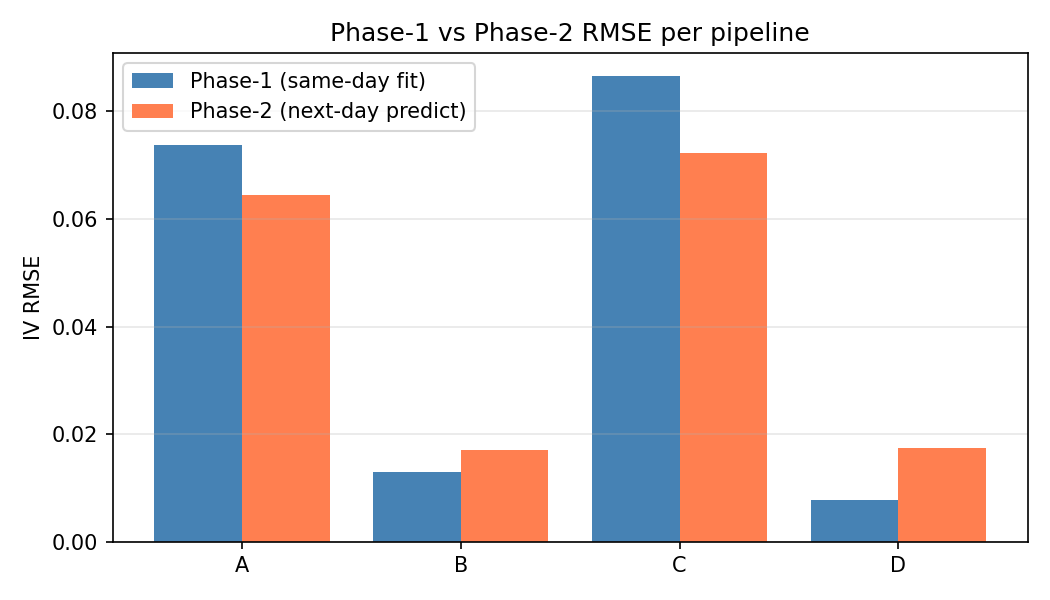
\includegraphics[width=\linewidth]{01_headline_rmse.png}
  \caption{IV-domain RMSE.}
\end{subfigure}
\begin{subfigure}[t]{0.49\linewidth}
  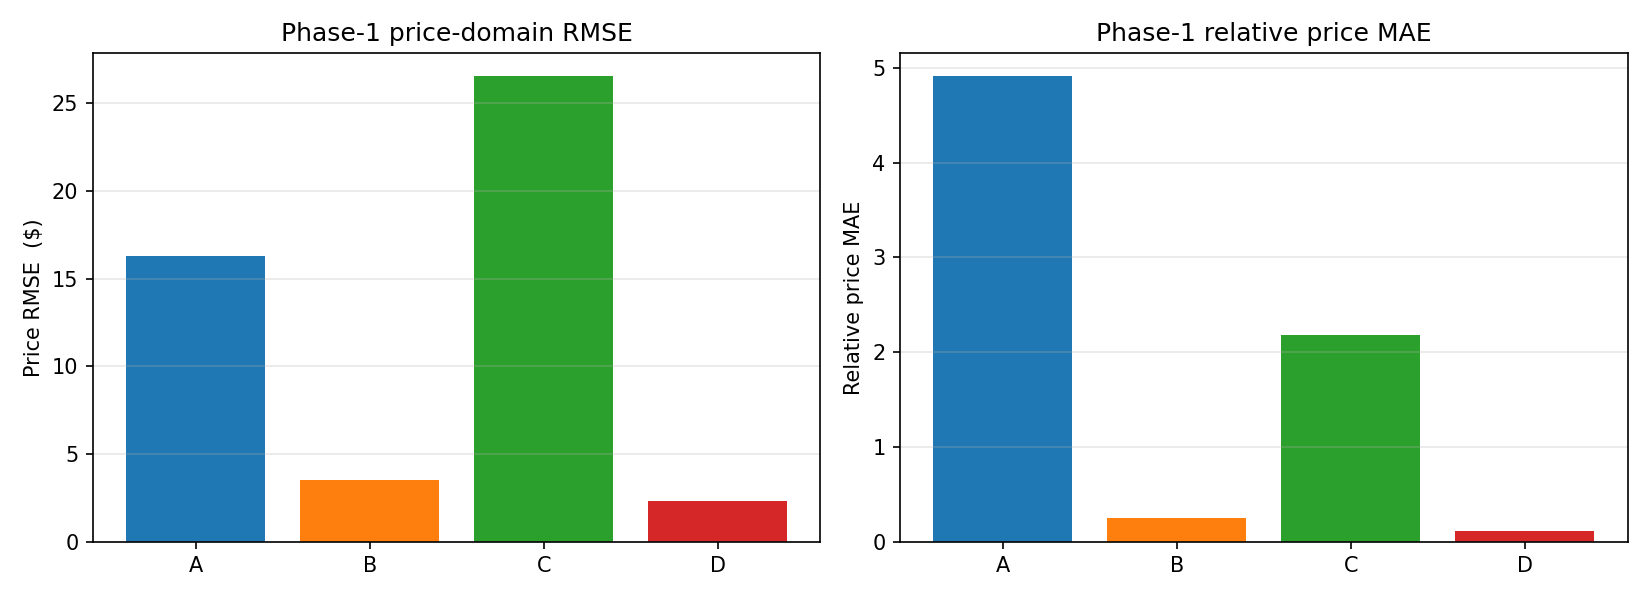
\includegraphics[width=\linewidth]{07a_price_headline.png}
  \caption{Price-domain RMSE.}
\end{subfigure}
\caption{Headline results across the four pipelines.}
\label{fig:headline}
\end{figure}

\subsection{IV-domain takeaways}

(i)~SSVI is the best on Phase-1 by a wide margin (RMSE
$0.0077$, half of HyperIV's $0.0131$). This is consistent with the
intuition that a five-parameter parametric surface, calibrated separately
to every day, has just enough flexibility to interpolate the typical SPX
smile while the no-arbitrage constraints regularise away the noise that a
neural net would otherwise overfit. (ii)~HyperIV is a close runner-up; on
Phase-2 it is essentially indistinguishable from SSVI ($0.0170$ vs.\
$0.0174$ RMSE), \emph{despite never having seen the test day at training
time}, simply because once a sensible reference set is provided, a single
forward pass produces the per-day weights. (iii)~The two price-domain
pipelines (ISNN, HyperISNN) are almost an order of magnitude worse in IV.
ISNN's $0.0737$ Phase-1 RMSE is, somewhat embarrassingly, \emph{worse than
predicting the previous day's IV} ($\Delta = +0.092$, positive is bad).

\subsection{Why price-domain hard-constrained nets do worse, even in their
home court}

Look at \cref{tab:price_headline}: ISNN reports a Phase-1 \$RMSE of
\$16.30 in its own native domain --- the same domain it was \emph{trained
to fit}. Meanwhile HyperIV, which is trained on IV and only sees prices
through a Black--Scholes inversion at evaluation time, posts \$3.51, and
SSVI posts \$2.35. The mechanism is the moneyness asymmetry of the loss:
ISNN-style models fit normalized call prices $C_{\mathrm{norm}}$ with MSE,
and deep ITM calls have intrinsic value pushing $C_{\mathrm{norm}}$
towards $1$, while OTM calls live near $0$. MSE thus over-weights ITM
intrinsic value (where there is no information) and under-weights the
volatility skew embedded in OTM prices. A small relative error on a deep
ITM normalized price is a large absolute dollar error after multiplying
back by spot.

By contrast, IV is on a natural common scale ($\sim$$0.1$--$0.8$) across
moneyness, so MSE on IV implicitly equalises the contribution of every
contract to the loss. When that IV is then BS-priced, the resulting dollar
errors are small \emph{on average and at the extremes}, because the BS
formula's vega is itself moneyness-dependent in the same way the
information content is.

A practical corollary, useful for anyone using ISNN downstream: do not
read prices directly off the ISNN head. Use the network's surface only to
extract IV (by inverting BS contract by contract) and then re-price; this
is more accurate even though it sounds redundant.

\begin{figure}[H]
\centering
\begin{subfigure}[t]{0.49\linewidth}
  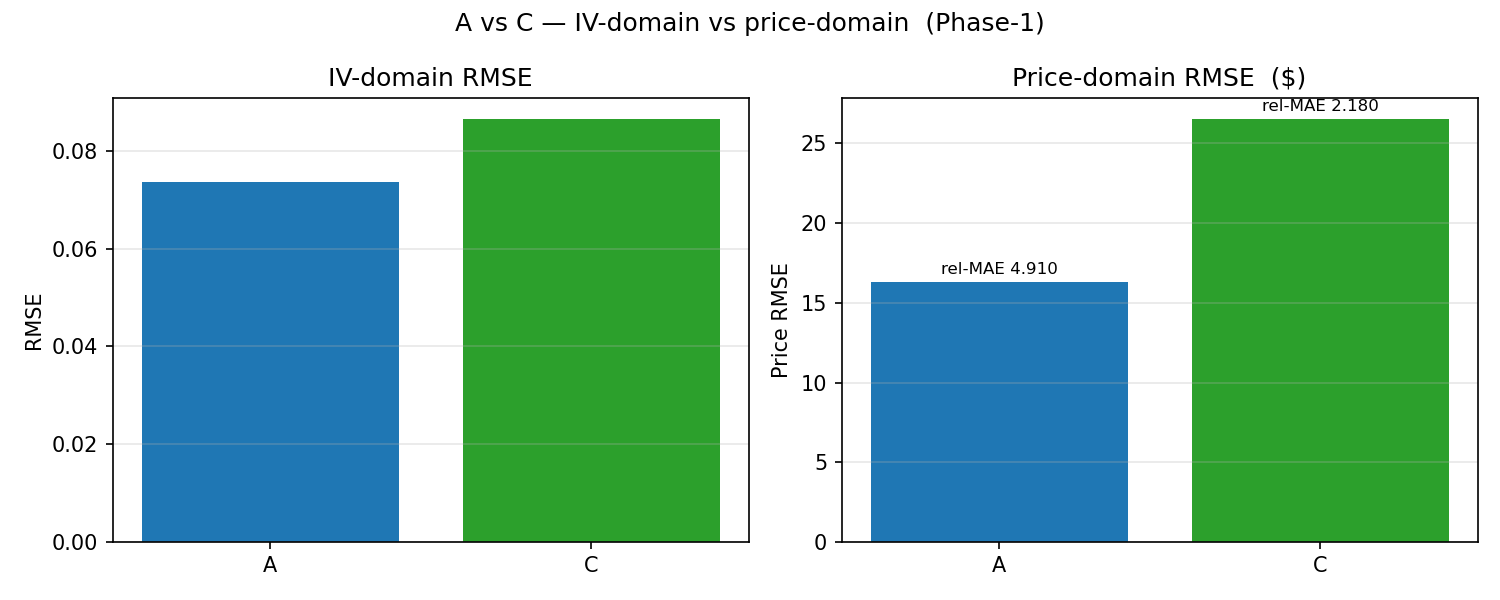
\includegraphics[width=\linewidth]{07b_price_iv_AC.png}
  \caption{Native price vs.\ BS-priced IV head, Pipelines A and C.}
\end{subfigure}
\begin{subfigure}[t]{0.49\linewidth}
  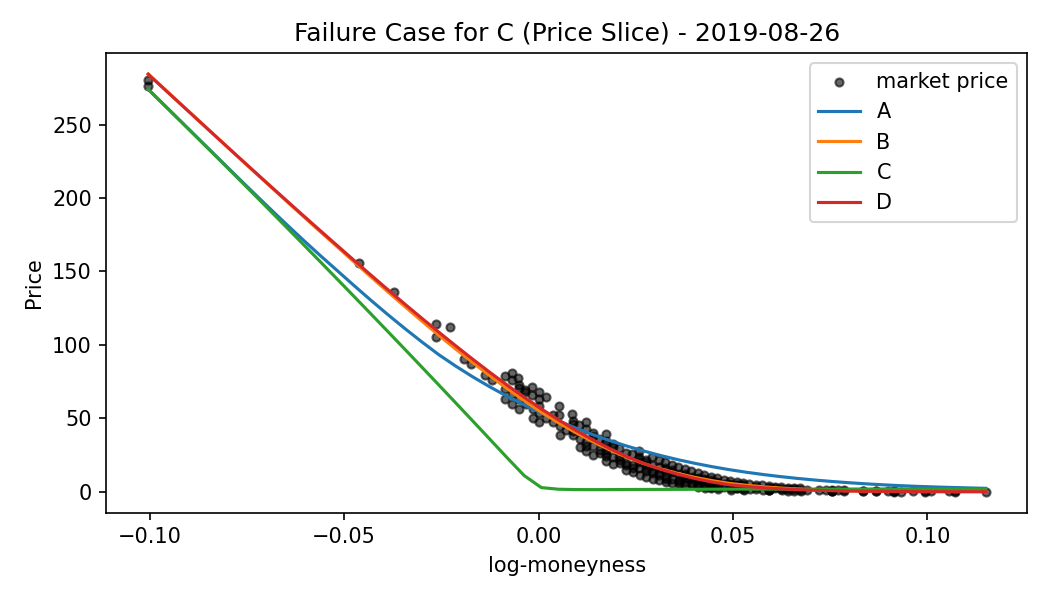
\includegraphics[width=\linewidth]{08_failure_case_price_2019-08-26.png}
  \caption{Failure-case slice on 2019-08-26.}
\end{subfigure}
\caption{Diagnostics for the price-domain failure of ISNN and HyperISNN.
Even on the loss they were trained on, the dollar error is large because
the MSE on normalized price over-weights ITM intrinsic value.}
\label{fig:price_failure}
\end{figure}

\subsection{Surfaces, slices, and bucket diagnostics}

\begin{figure}[H]
\centering
\begin{subfigure}[t]{0.24\linewidth}
  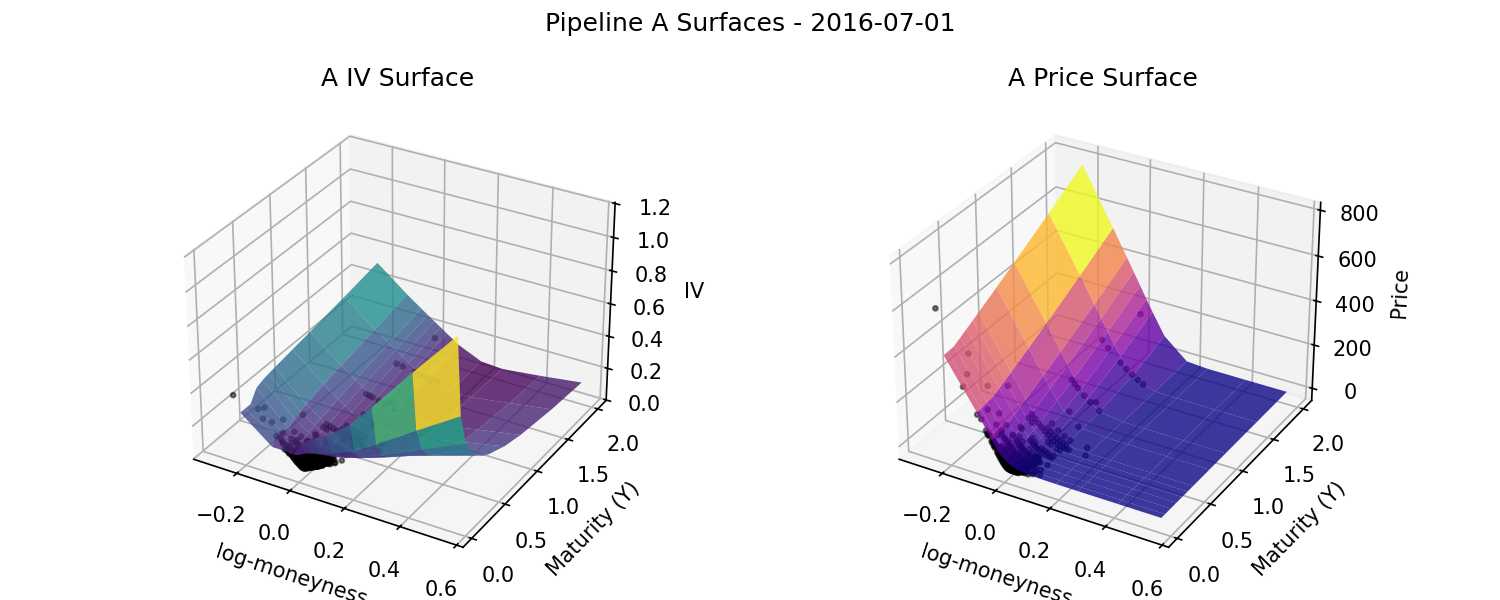
\includegraphics[width=\linewidth]{09_3d_surfaces_A.png}
  \caption{ISNN}
\end{subfigure}
\begin{subfigure}[t]{0.24\linewidth}
  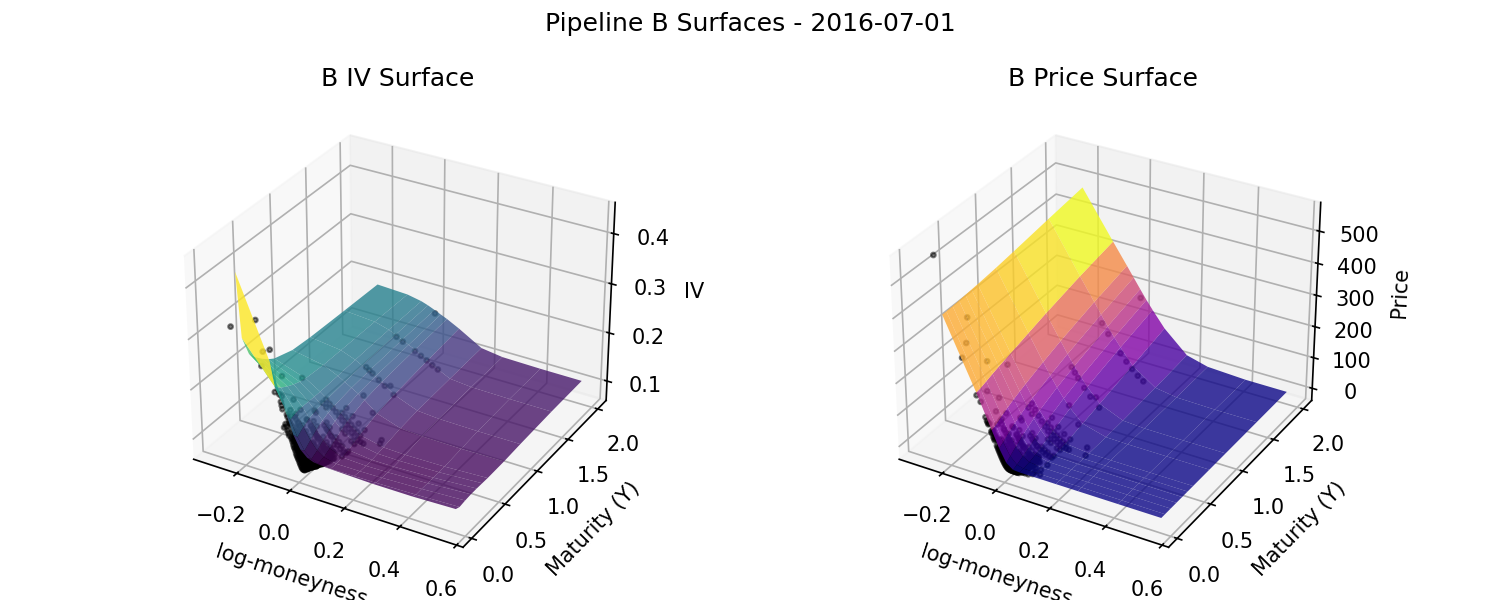
\includegraphics[width=\linewidth]{09_3d_surfaces_B.png}
  \caption{HyperIV}
\end{subfigure}
\begin{subfigure}[t]{0.24\linewidth}
  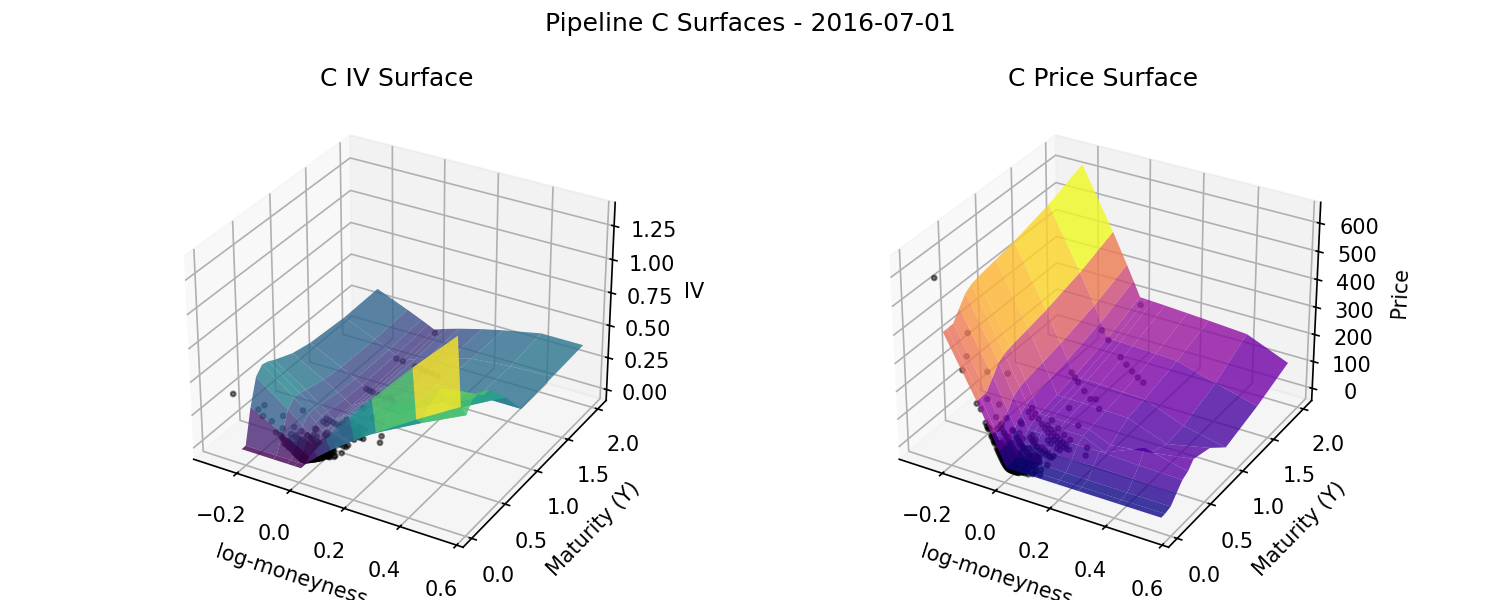
\includegraphics[width=\linewidth]{09_3d_surfaces_C.png}
  \caption{HyperISNN}
\end{subfigure}
\begin{subfigure}[t]{0.24\linewidth}
  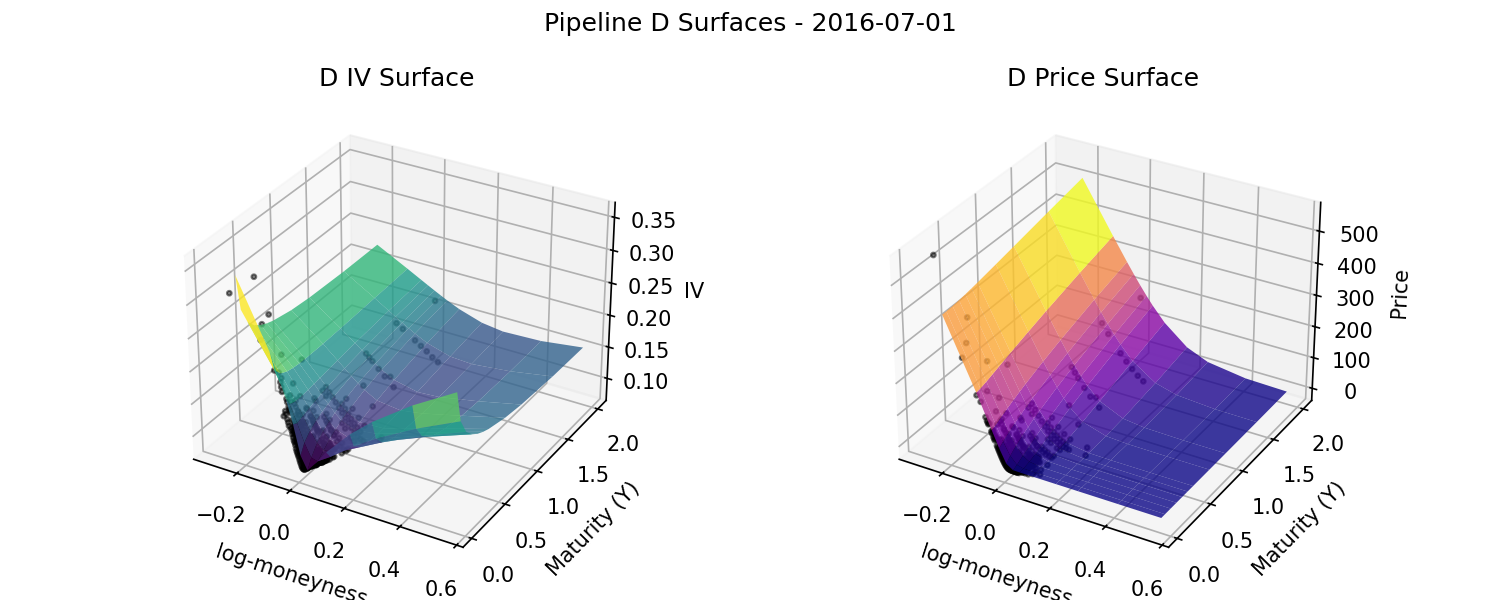
\includegraphics[width=\linewidth]{09_3d_surfaces_D.png}
  \caption{SSVI}
\end{subfigure}
\caption{Phase-1 IV surfaces on a representative day. The HyperIV and
SSVI surfaces are visibly tighter and more skewed; ISNN/HyperISNN over-
smooth the wings.}
\label{fig:3d_surfaces}
\end{figure}

\begin{figure}[H]
\centering
\begin{subfigure}[t]{0.32\linewidth}
  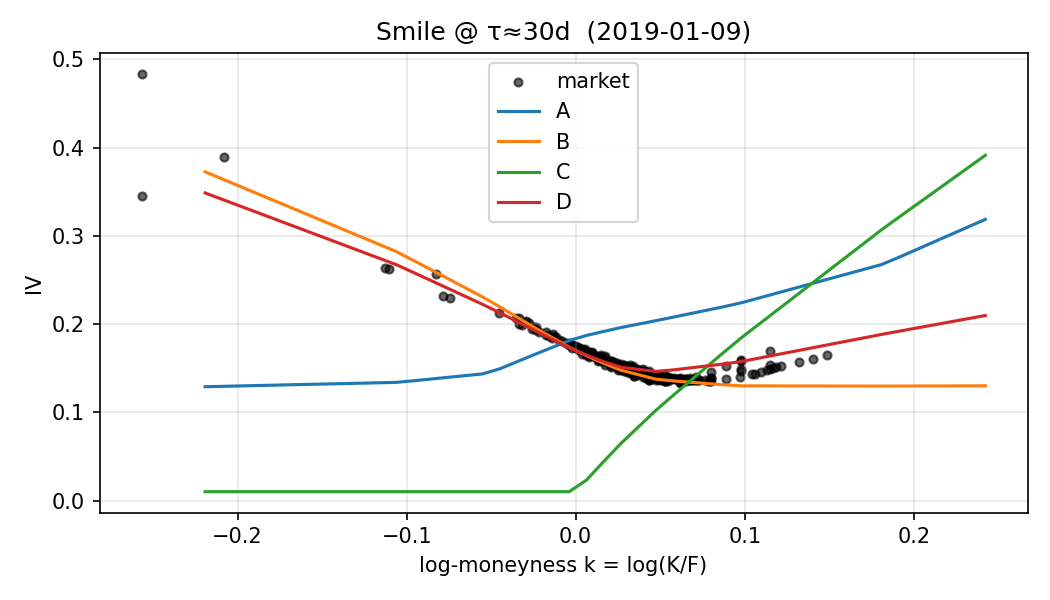
\includegraphics[width=\linewidth]{slice_smile_2019-01-09.png}
  \caption{2019-01-09 smile slice.}
\end{subfigure}
\begin{subfigure}[t]{0.32\linewidth}
  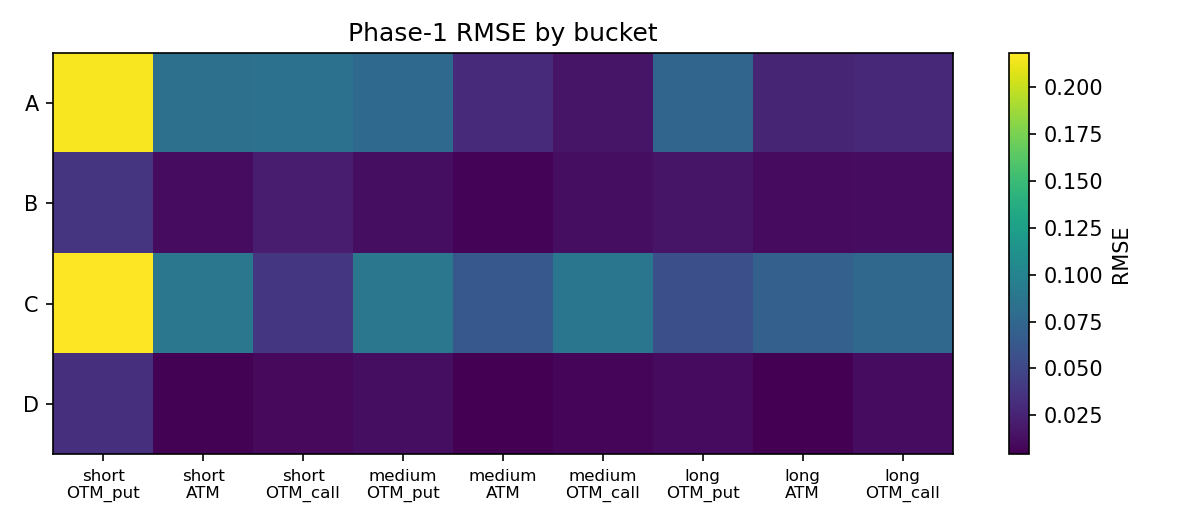
\includegraphics[width=\linewidth]{03a_buckets_phase1.png}
  \caption{Phase-1 by moneyness $\times$ maturity bucket.}
\end{subfigure}
\begin{subfigure}[t]{0.32\linewidth}
  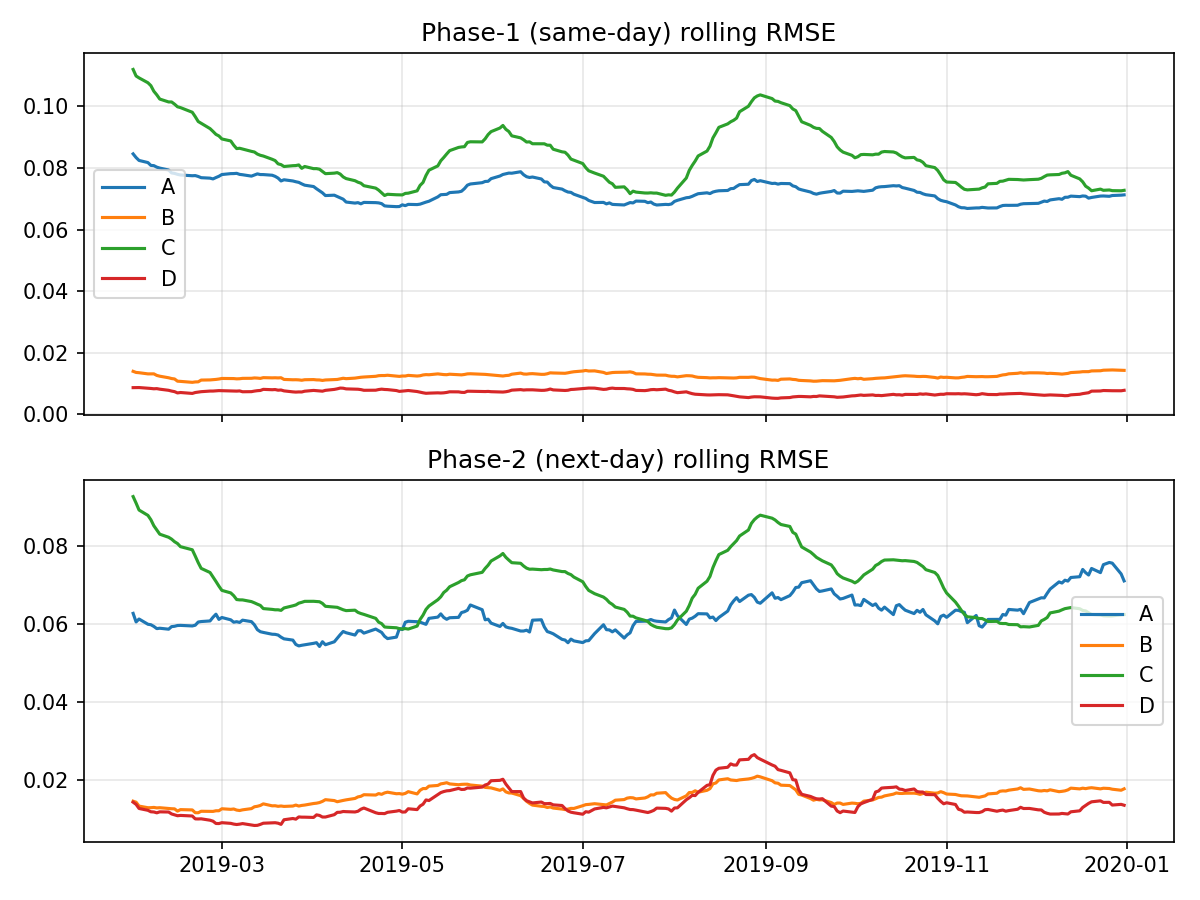
\includegraphics[width=\linewidth]{06_rolling_rmse.png}
  \caption{Rolling test-set RMSE through 2019.}
\end{subfigure}
\caption{Per-slice and per-bucket diagnostics. SSVI dominates uniformly;
HyperIV is competitive everywhere; ISNN/HyperISNN miss the wings.}
\label{fig:slices}
\end{figure}

\subsection{HyperISNN vs.\ ISNN: less accurate, but much faster}

HyperISNN is uniformly less accurate than ISNN (Phase-1 IV RMSE $0.0865$
vs.\ $0.0737$, Phase-1 \$RMSE $26.52$ vs.\ $16.30$). The cause is a
combination of: (i)~the residual weight generator must hit the same
positive softplus targets across thousands of days with a single shared
$W_{\mathrm{base}}$, so the per-day modulation $\alpha \odot \omega$
cannot fully compensate; and (ii)~the warm-up phase converges to a
``mean'' ISNN that the hyper-network is then asked to perturb by a small
amount, leaving the model in a basin where butterfly-strict positivity
limits the surface flexibility.

In return, HyperISNN inherits HyperIV's amortisation argument: at
inference, a single Set-Transformer forward pass produces the entire
ISNN-2 weight vector, and a single ISNN evaluation produces the surface.
There is no per-day fit. ISNN, by contrast, requires a $2{,}000$-epoch
Adam fit per day. So HyperISNN trades $\sim$$15\%$ relative IV accuracy
for two-to-three orders of magnitude in inference cost.

\subsection{Wall-clock: HyperIV inference vs.\ SSVI per-day fit}

\begin{table}[H]
\centering
\small
\begin{tabular}{lrr}
\toprule
Operation (single thread, M-series CPU) & median (ms / day) & p95 (ms / day) \\
\midrule
SSVI per-day fit (L-BFGS-B, $10$ restarts)            & $154.5$  & $241.6$ \\
HyperIV: encoder only ($g_\theta(Z_t) \to \omega_t$)  & $0.147$  & $0.604$ \\
HyperIV: encoder + market-quote evaluation            & $0.282$  & $1.067$ \\
\bottomrule
\end{tabular}
\caption{Wall-clock per-day cost over $30$ test days, measured by
\texttt{bench\_timing.py}. Median speedup of HyperIV inference vs.\ SSVI
per-day calibration is $\approx 547\times$.}
\label{tab:timing}
\end{table}

The $\sim$$500\times$ speedup is the central operational advantage of
HyperIV over SSVI: amortising the calibration into a one-time training
cost reduces a $\sim$$160$\,ms per-day non-convex fit to a sub-millisecond
forward pass, with only a small accuracy concession (Phase-1 IV RMSE
$0.0131$ vs.\ $0.0077$). For a desk that re-prices intraday, or any
backtest that loops over years of days, this is the difference between a
calibration-bound pipeline and an inference-bound one.

\subsection{Phase-2 with VolGAN: better Phase-1 surfaces beget better
next-day forecasts}

\begin{figure}[H]
\centering
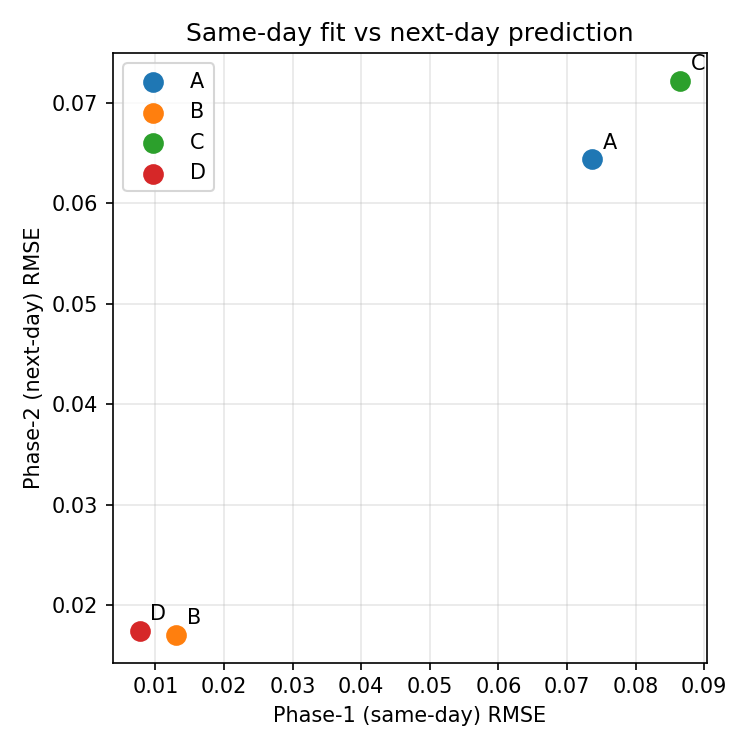
\includegraphics[width=0.55\linewidth]{02_p1_vs_p2_scatter.png}
\caption{Phase-2 RMSE plotted against Phase-1 RMSE for the four pipelines.
The relationship is monotone: more accurate Phase-1 fits become more
accurate next-day VolGAN forecasts.}
\label{fig:p1_vs_p2}
\end{figure}

This is the unsurprising-but-important finding for any practitioner who
plans to plug a deep IV model into a downstream generator: VolGAN is
\emph{not} a regulariser. Whatever errors live in the Phase-1 surface are
absorbed by the GAN training distribution and propagate into the Phase-2
forecast. SSVI ranks first in both, HyperIV second in both, ISNN /
HyperISNN last in both, and the ordering is preserved across the
Phase-1 $\to$ Phase-2 transition.

% =============================================================================
\section{Summary of Final Outcome}
\label{sec:summary}

We brought Pipelines A--D under one roof and made the following findings:

\begin{enumerate}[leftmargin=*,itemsep=2pt]
  \item \textbf{Native price-domain hard-constrained networks (ISNN,
        HyperISNN) underperform native volatility-domain models
        (HyperIV, SSVI) in every metric we measured.} They are less
        accurate in IV (an order of magnitude on Phase-1), and --- the
        more surprising result --- less accurate \emph{in their own price
        domain} than the IV-domain models that go through an extra BS
        inversion. The mechanism is the moneyness asymmetry of MSE on
        normalized prices.
  \item \textbf{SSVI is the most accurate model overall.} Its
        five-parameter surface, fit by L-BFGS-B with multiple restarts and
        constrained to the Gatheral--Jacquier no-arbitrage region, hits
        the lowest Phase-1 IV RMSE ($0.0077$) and the lowest Phase-2 IV
        RMSE ($0.0174$). The cost is a $\sim$$160$\,ms per-day fit (single
        thread, M-series CPU).
  \item \textbf{HyperIV is essentially as good in Phase-2 and
        $\sim$$500\times$ faster.} Once trained, a single forward pass
        through the Set-Transformer encoder produces the per-day IV-MLP
        weights, and the resulting surface is competitive with SSVI on
        the next-day stress test. This is the practical case for
        amortised hyper-networks in finance: the calibration cost is paid
        once, off-line, and then any number of days can be priced on the
        margin.
  \item \textbf{HyperISNN trades accuracy for speed in the price-domain
        family.} It is less accurate than per-day ISNN, but inherits
        HyperIV's inference budget; both Phase-1 and Phase-2 numbers are
        worse than ISNN, but by a constant factor. The architecture is a
        useful template for ``how to amortise a hard-constrained
        per-day fitter'', even though, in this study, the cost in
        accuracy outweighs the gain in speed.
  \item \textbf{Better Phase-1 surfaces yield better Phase-2 forecasts.}
        The Phase-2 ranking (under VolGAN) is the same as the Phase-1
        ranking. Practitioners should not expect a downstream generator
        to compensate for an inaccurate surface model.
\end{enumerate}

\paragraph{Recommendations.}
For batch backtesting where per-day calibration cost is a bottleneck, use
HyperIV. For one-off pricing on a single day where calibration cost is
amortised over many quotes, use SSVI. Avoid native ISNN price outputs in
production; if ISNN-style models must be used (for the architectural
arbitrage guarantee), invert their prices to IV and re-price through BS.

% =============================================================================
\bibliographystyle{plainnat}
\bibliography{paper}

% =============================================================================
\appendix

\section{Hyperparameter tables}
\label{app:hp}

\begin{table}[H]
\centering
\small
\begin{tabular}{lll}
\toprule
& Pipeline A (ISNN) & Pipeline B (HyperIV) \\
\midrule
Architecture          & ISNN-2, $H{=}64$, $L{=}3$               & SetTransformer $d{=}128$, $2$ layers, $2$ heads \\
Target output         & Normalized call $C/S$                  & IV $\iv$ \\
Loss                  & MSE($C/S$)                              & MSE($\iv$) + cal + butterfly + Durrleman \\
Optimizer             & Adam, LR $10^{-2}$                      & Adam, LR $10^{-3}$, cosine $\to 10^{-5}$ \\
Schedule              & $2{,}000$ epochs / day                  & $500$ epochs total, batch $128$ \\
Constraints           & Non-neg.\ weight clamp                  & Soft arb.\ penalties \\
Reference set         & ---                                     & $9$ contracts at $\Delta {\in} \{0.75, 0.5, 0.25\}$ \\
\bottomrule
\end{tabular}
\caption{Pipelines A and B hyperparameters.}
\end{table}

\begin{table}[H]
\centering
\small
\begin{tabular}{lll}
\toprule
& Pipeline C (HyperISNN) & Pipeline D (SSVI) \\
\midrule
Architecture          & SetTransformer $d{=}128$, $3$ layers, $4$ heads & 5-param Gatheral--Jacquier \\
Target network        & ISNN-2, $H{=}8$, $L{=}3$                          & --- \\
Weight scheme         & $W_{\mathrm{raw}} = W_{\mathrm{base}} + \alpha \odot \omega(Z)$ & --- \\
$\alpha$ init         & $0.1$ per parameter                              & --- \\
Loss                  & MSE($C/S$) + upper + var penalties               & ATM-weighted MSE($\iv$) \\
Optimizer             & AdamW, LR $3\times 10^{-4}$, wd $10^{-4}$        & L-BFGS-B \\
Schedule              & $10{,}000$ steps, cosine warm restart $T_0{=}1000$ & $10$ random restarts \\
Warm-up               & $500$ steps, $\alpha$ \& hypernet frozen         & --- \\
Batch                 & $32$ episodes / step                             & --- \\
Grad clip             & $1.0$                                            & --- \\
\bottomrule
\end{tabular}
\caption{Pipelines C and D hyperparameters.}
\end{table}

\section{Additional plots}
\label{app:plots}

\begin{figure}[H]
\centering
\begin{subfigure}[t]{0.32\linewidth}
  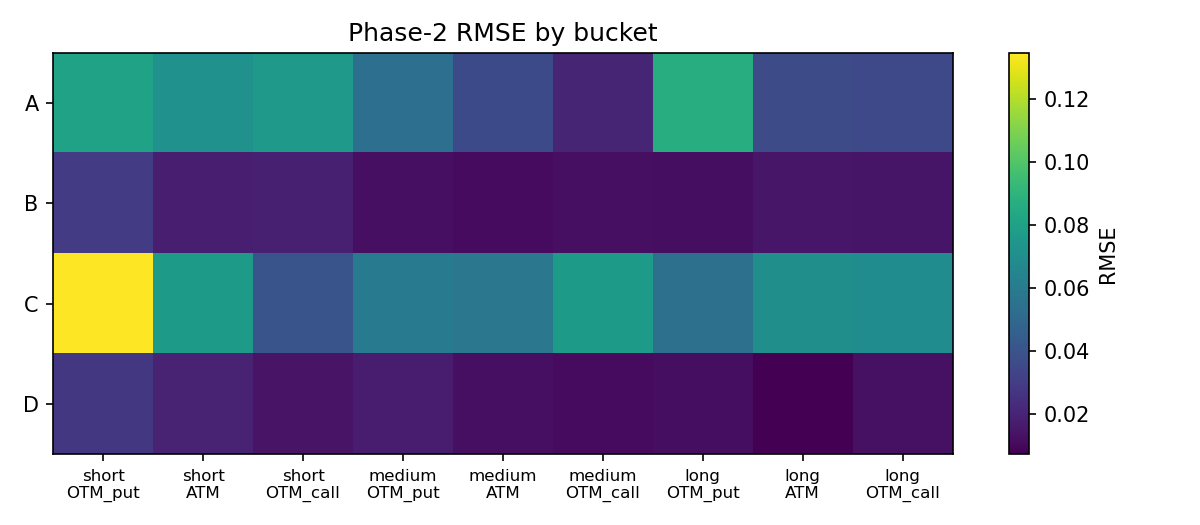
\includegraphics[width=\linewidth]{03b_buckets_phase2.png}
  \caption{Phase-2 buckets.}
\end{subfigure}
\begin{subfigure}[t]{0.32\linewidth}
  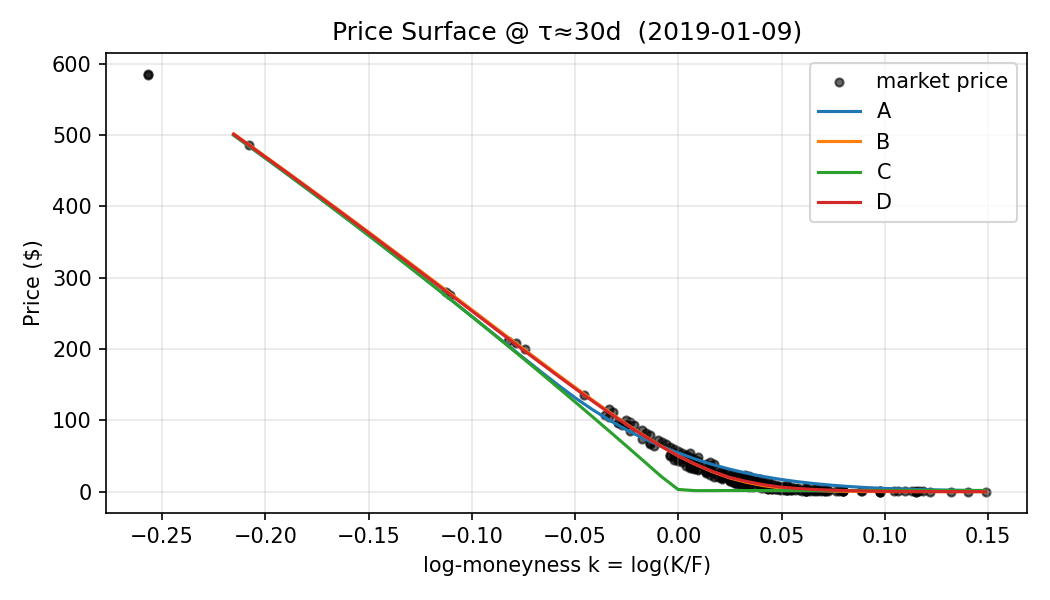
\includegraphics[width=\linewidth]{slice_price_2019-01-09.png}
  \caption{Price slice 2019-01-09.}
\end{subfigure}
\begin{subfigure}[t]{0.32\linewidth}
  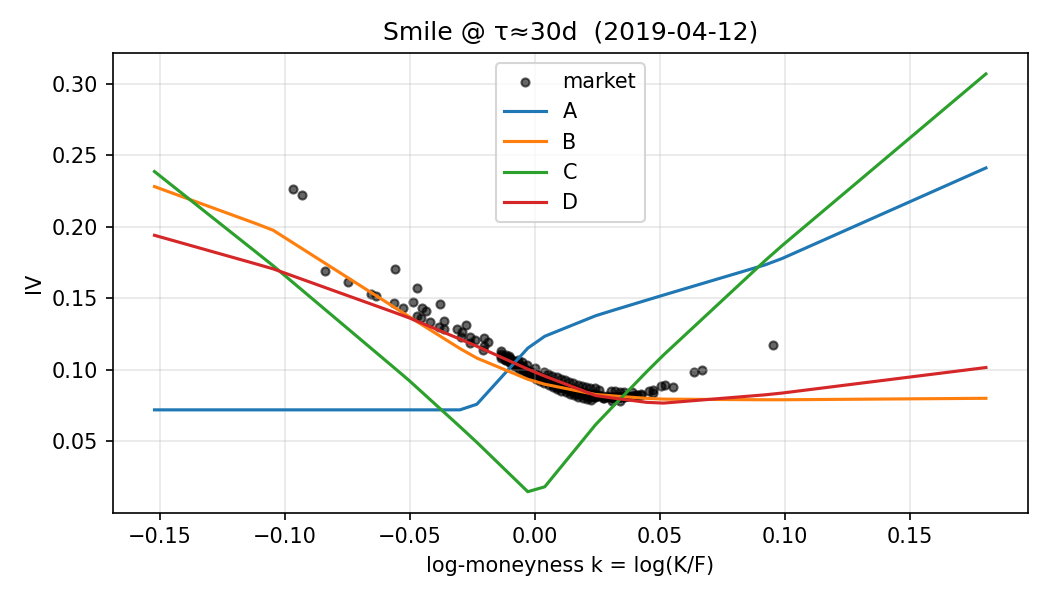
\includegraphics[width=\linewidth]{slice_smile_2019-04-12.png}
  \caption{Smile slice 2019-04-12.}
\end{subfigure}
\caption{Additional cross-pipeline diagnostics.}
\end{figure}

\begin{figure}[H]
\centering
\begin{subfigure}[t]{0.32\linewidth}
  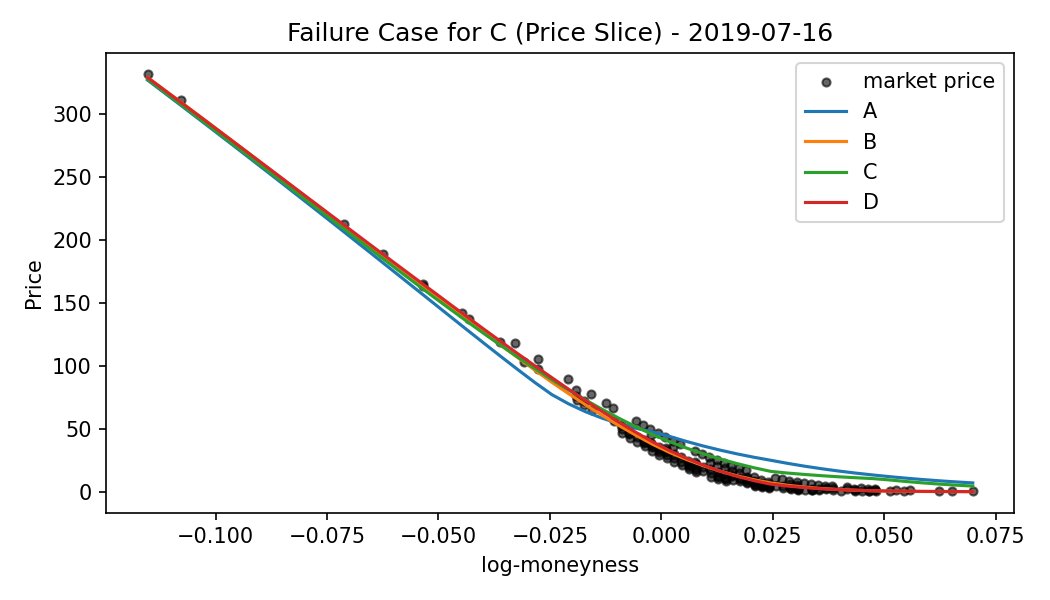
\includegraphics[width=\linewidth]{08_failure_case_price_2019-07-16.png}
  \caption{2019-07-16}
\end{subfigure}
\begin{subfigure}[t]{0.32\linewidth}
  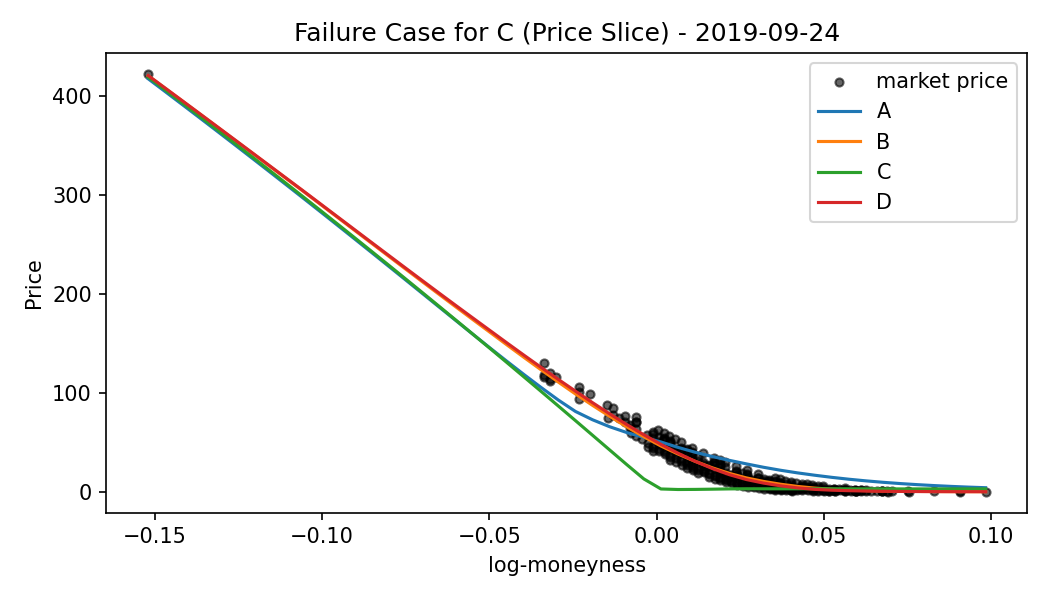
\includegraphics[width=\linewidth]{08_failure_case_price_2019-09-24.png}
  \caption{2019-09-24}
\end{subfigure}
\begin{subfigure}[t]{0.32\linewidth}
  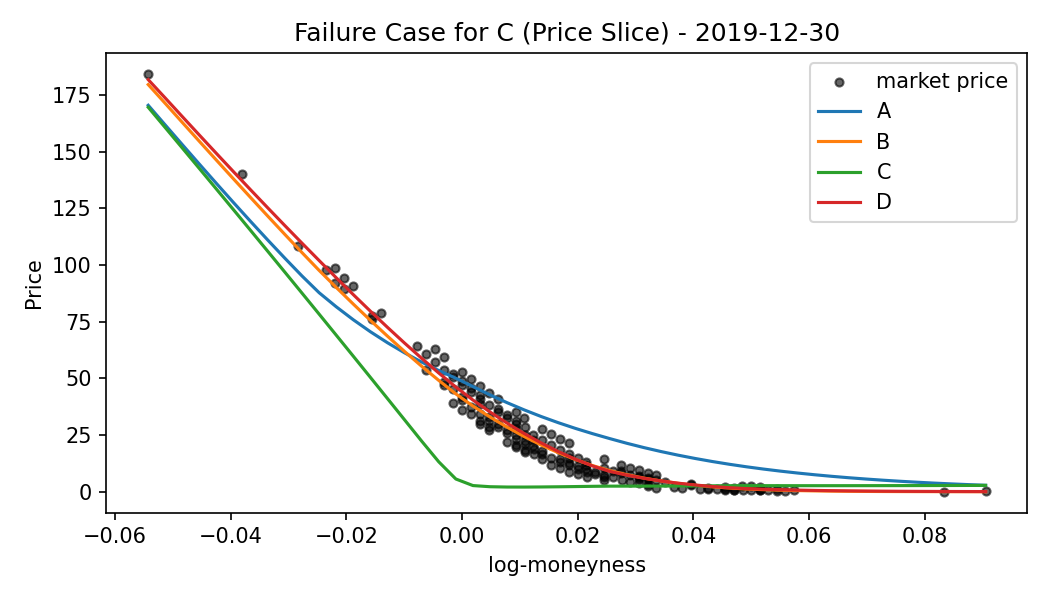
\includegraphics[width=\linewidth]{08_failure_case_price_2019-12-30.png}
  \caption{2019-12-30}
\end{subfigure}
\caption{Additional ISNN / HyperISNN price-domain failure cases.}
\end{figure}

\section{Reproducibility}
\label{app:repro}

All numbers in this report are produced from the \texttt{main\_project}
repository. The wall-clock benchmark in \cref{tab:timing} is reproduced
by:
\begin{verbatim}
PYTHONPATH=code_files python bench_timing.py
\end{verbatim}
which loads the unified test-set quotes and the trained HyperIV
checkpoint from \texttt{data/unified/}. Headline accuracy numbers in
\cref{tab:iv_headline} and \cref{tab:price_headline} come from the
unified evaluation harness in \texttt{code\_files/shared\_eval/} and are
mirrored in \texttt{data/unified/results/summary.md}. Plots are produced
by \texttt{code\_files/shared\_eval/plots.py} and live in
\texttt{plots/}.

\end{document}
